\section{Motivating scenarios}
\label{sec:sidekick:motivating}

\begin{figure}[t]
	\centering
	% \includegraphics[width=\linewidth]{figures/sc-legend.pdf}\\
	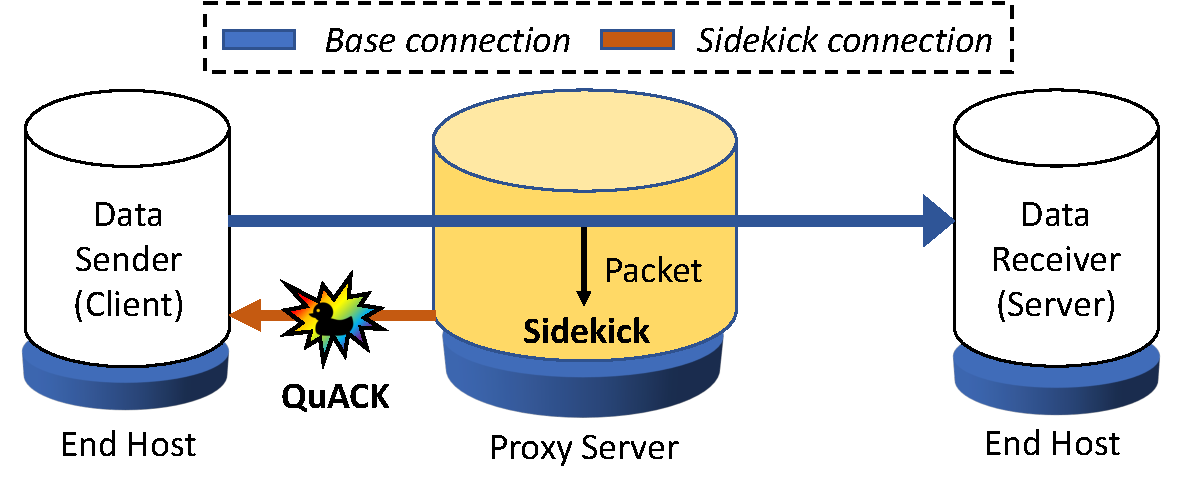
\includegraphics[width=\linewidth]{figures/sc_protocol.pdf}%
\caption{The proxy generates quACKs, in-network acknowledgments, based on
the opaque packets it observes in the base protocol. It quACKs to an end
host, the data sender, which sends or resends packets on the base protocol as a result.
Although we only show one side of the connection, the \sys could assist
either end host of a bidirectional flow.
\vspace{-0.4cm}
}
\label{fig:sc-protocols}
\end{figure}


We focus on three scenarios where end hosts benefit from in-network assistance.
In each one, a proxy server provides feedback, called a quACK, to an end host:
the data sender (\Cref{fig:sc-protocols}). Recall that a quACK is a
``cumulative ACK + selective ACK'' over encrypted sequence numbers. The data
sender uses this feedback to influence its behavior on the base connection,
without altering the wire format.

To be clear: the Sidekick protocol is not tied to a specific base protocol
nor to how the end hosts use the quACK information. The base protocol does not
need to be reliable, nor to have unique datagrams---we implemented and evaluated
the same Sidekick protocol and the same middlebox behavior across the different
scenarios in this paper.

\subsection{Low-latency media retransmissions}
\label{sec:sidekick:motivating:media}

Consider a train passenger using on-board Wi-Fi to have a low-latency audio
conversation, using WebRTC/SRTP~\cite{rfc8834webrtc}, with a friend. The
end-to-end network path contains a low-latency, high-loss ``near'' path
segment (the Wi-Fi hop) followed by a high-latency, low-loss ``far'' path
segment (the cellular and wired path over the Internet). The friend probably
suffers from poor connection quality, experiencing drops in the audio stream or
high de-jitter buffer delays from waiting for retransmitted packets to be
played in order (\Cref{fig:media} in emulation, \Cref
{fig:real-world:scenario1} in real world).

In the Sidekick approach, a Sidekick on the Wi-Fi access point sends quACKs to the audio
application on the user's laptop, assisting the base connection's data sender.
The sender uses quACKs to retransmit packets sooner than they would have using
negative acknowledgments (NACKs) from the receiver. The end result is similar
to the effect of prior PEPs, such as Snoop~\cite{balakrishnan1995snoop} and
Milliproxy~\cite{polese2017milliproxy}, that leverage TCP's cleartext sequence
numbers to trigger early retransmission on lossy wireless paths.

\subsection{Emulating split congestion control in an HTTP/3 file upload}
\label{sec:sidekick:motivating:http}

Consider the same train passenger as before but uploading a large file over the
Internet with a reliable transport protocol. If the protocol were TCP, the
train could deploy a split TCP PEP at the access point. The split connection
allows quick detection and retransmission of dropped packets on the lossy Wi-Fi
segment, while opening up the congestion window on the high-latency cellular
segment.

However, opaque transport protocols like QUIC can't benefit from (nor be harmed
by) connection-splitting PEPs. Without a PEP, QUIC relies on end-to-end
mechanisms over the entire path to detect losses, recover from them, and adjust
the congestion-control behavior. This leads to reduced upload speeds
(\Cref{fig:baseline-line} in emulation, \Cref{fig:real-world:scenario2} in real world).

With help from the same Sidekick PEP, the QUIC sender combines information from
quACKs and end-to-end ACKs to emulate the congestion-control behavior of a
split TCP connection (\Cref{sec:sidekick:sender}). The
application considers whether packets are lost on the near or far path
segments, and adjusts the congestion window accordingly while respecting the
opacity of the end-to-end base connection. The application also retransmits the
packet as soon as the loss has been detected.

The only guarantee the proxy makes to the sender via the quACK is that it has
received some packets. To respect the end-to-end reliability contract with the
receiver, the sender does not delete packets that may need to be transmitted
until it receives an ACK, even if the packet has been quACKed.

\subsection{Battery-saving ACK reduction}
\label{sec:sidekick:motivating:ack-reduction}

Now consider a battery-powered device downloading a large file from the
Internet. To reduce how often the receiver's
radio needs to wake up, saving energy, the base connection can reduce the
frequency of end-to-end ACKs the device sends.
ACK reduction has also been shown to improve performance by reducing collisions
and contention over half-duplex links~\cite{custura2023reducing,li2020tack}.
The ACK frequency can be configured with a TCP kernel setting or proposed
QUIC extension~\cite{ietf-quic-ack-frequency-07}.

However, ACK reduction can also degrade throughput~\cite{custura2023reducing,custura2020impact}
(\Cref{fig:ack-reduction} in emulation).
The sender receives more delayed feedback about loss, and has to carefully
pace packets to avoid bursts in the large delay between ACKs.
One proposal has the PEP acknowledge packets on behalf of the
receiver~\cite{kliazovich2012arqproxy}, leveraging cleartext TCP sequence
numbers, but it does not apply to opaque transport protocols.

In this case, a Sidekick at the Wi-Fi access point (or a cellular base station)
quACKs to the sender on behalf of the receiver. The receiver still occasionally
wakes up its radio to send ACKs, but the sender uses the more frequent quACKs
to advance its flow-control and congestion-control windows.

The sender respects the end-to-end reliability contract by only deleting packets
in response to ACKs, but disregards the receiver's flow control by using quACKs
to advance the flow-control window. If the sender only used ACKs to advance the
window, it would waste time waiting between ACKs to send packets with too small
a window, and need to pace sent packets on receiving a large ACK with too large
a window.
